\documentclass[a4paper,10pt]{scrreprt}
\usepackage{pgfplots}
\usepackage[utf8]{inputenc}
\usepackage[french]{babel}
\usepackage{rotating}
% \usepackage[tmargin=1in,bmargin=1in,lmargin=1in,rmargin=1in]{geometry}
\usepackage{wordlike}
\pgfplotsset{compat=1.9}
\usepackage{xcolor}
\usepackage{titlesec}
\usepackage{wrapfig}
\usepackage{array}
\usepackage{geometry}
\usepackage{textcomp}
\usepackage{pgfgantt}

\newcolumntype{L}[1]{>{\raggedright\let\newline\\\arraybackslash\hspace{0pt}}m{#1}}
\newcolumntype{C}[1]{>{\centering\let\newline\\\arraybackslash\hspace{0pt}}m{#1}}
\newcolumntype{R}[1]{>{\raggedleft\let\newline\\\arraybackslash\hspace{0pt}}m{#1}}

% \definecolor{MSDarkBlue}{rgb}{.1,.15,.25}
\definecolor{MSBlue}{rgb}{.204,.353,.541}
\definecolor{MSLightBlue}{rgb}{.31,.506,.741}
% \newfontfamily\subsubsectionfont[Color=MSLightBlue]{Times New Roman}
% \titleformat*{\chapter}{\huge\bfseries\sffamily\color{MSDarkBlue}}
\titleformat*{\section}{\Large\bfseries\sffamily\color{MSBlue}}
\titleformat*{\subsection}{\large\bfseries\sffamily\color{MSLightBlue}}
\titleformat*{\subsubsection}{\bfseries\sffamily\color{MSLightBlue}}


% Title Page
% \title{SocaDB, gestion de données \\ pour le collaboratif temps-réel \\ entre objets, algorithmes et utilisateurs}
% \author{Hugo Leclerc}

\begin{document}

% --------------------------------------------------------------------------------------------------------------------------------
% ------------------------------------------------------ page de titre -----------------------------------------------------------
% --------------------------------------------------------------------------------------------------------------------------------
\thispagestyle{empty}

\newgeometry{bottom=0.0cm}

\hspace{2cm}
\vspace{2cm}

\begin{center}
    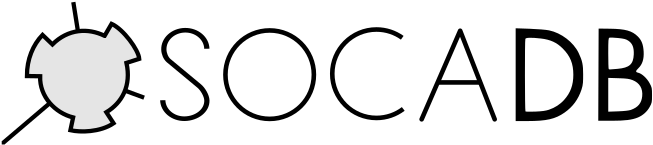
\includegraphics[width=0.5\paperwidth]{img/logo_wo_test.pdf}
    \vspace{3cm}
    
    %     \bfseries
    \sffamily
    \huge
    le Système de Gestion de Bases de Données \\ pour la \textbf{\color{MSBlue}collaboration temps-réel} \\ entre \textbf{\color{MSLightBlue}utilisateurs, algorithmes et objets}

    \vspace{2cm}
    \Large
    Concours national de création d’entreprises innovantes\\Catégorie émergence
    
    \vspace{0.5cm}
    \Large
    Hugo LECLERC
    
    \vfill
    %\vspace{2cm}
    
    % \makebox[\textwidth]{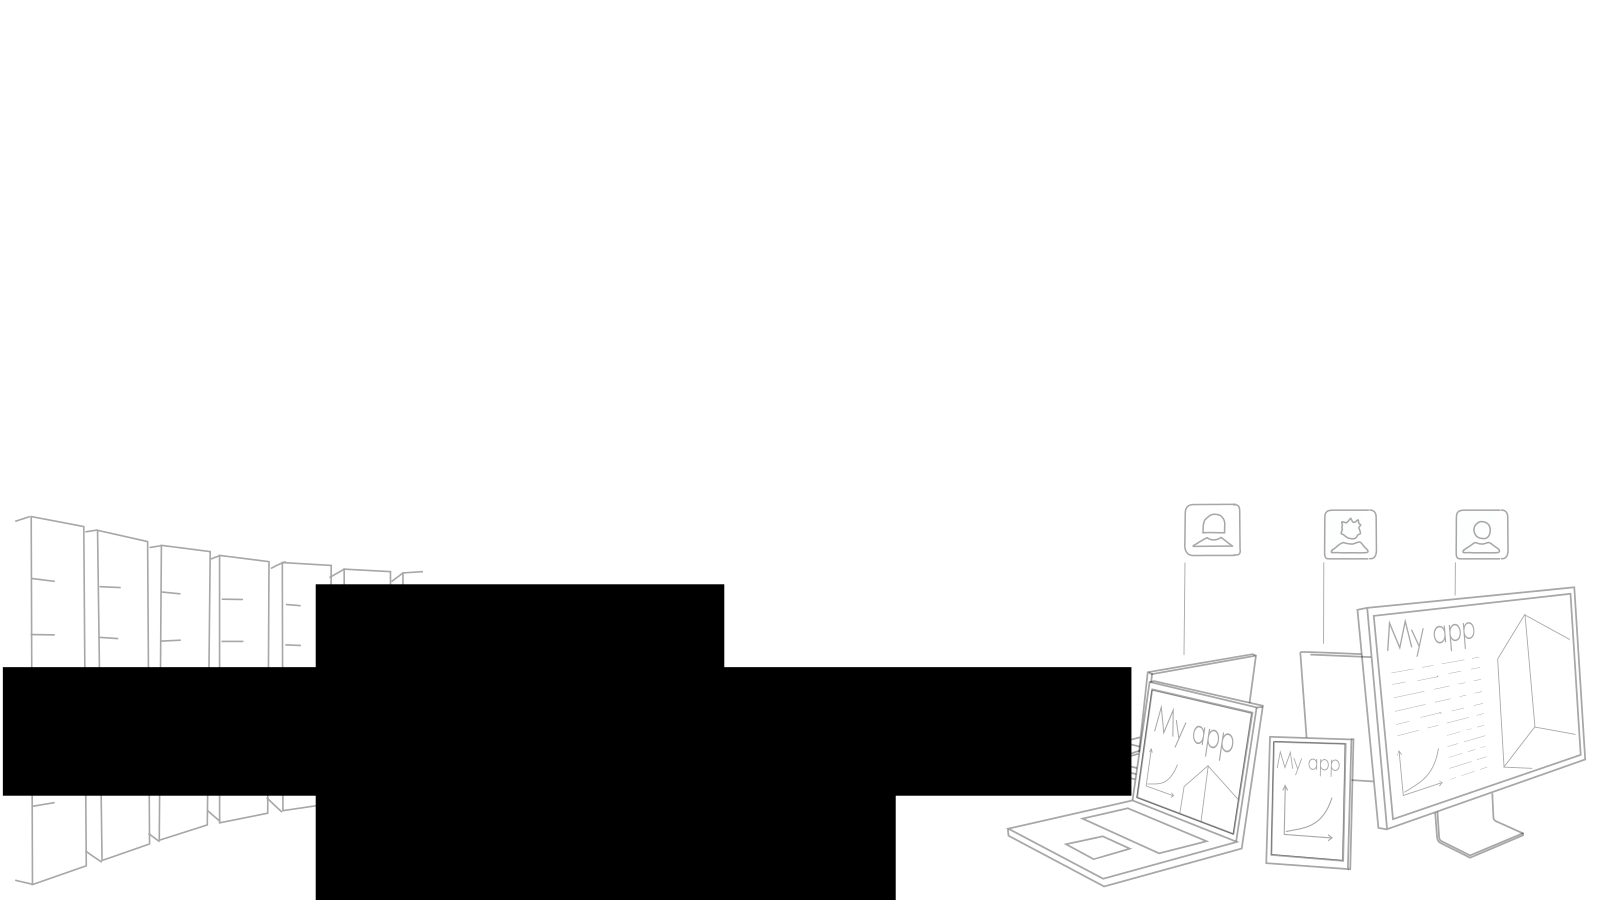
\includegraphics[width=\paperwidth]{img/main_image.pdf}}
\end{center}

\restoregeometry

% --------------------------------------------------------------------------------------------------------------------------------
% --------------------------------------------------------------------------------------------------------------------------------
% --------------------------------------------------------------------------------------------------------------------------------
\chapter*{Résumé opérationnel}

    \section*{Description du produit}
    
        SocaDB est une base de données conçue en fonction des besoins réels des développeurs d'applications interactives modernes. Les modèles de programmation qui en découlent permettent d'\textbf{accélérer de façon significative} la production de ce genre de programmes, en particulier si présence de \textbf{collaboratif temps-réel} (possibilité d'éditer à plusieurs le même document en même temps) et de \textbf{multiples composants} (objets connectés, interfaces utilisateurs, programmes de services, etc..).
    
        La prise en compte du contexte global a par ailleurs permis de proposer des solutions pour \textbf{réduire considérablement les besoins en termes de ressources énergétiques et matérielles}.
    
        \medskip
        Ce produit se présente sous la forme d'une logiciel libre. Les revenus principaux seront ceux de l'expertise : production d'applications utilisant SocaDB, développements ad-hoc, formation, contrats de maintenance et location de matériel pré-installé.
    
    \section*{Présentation de l'équipe}

        Le porteur de projet, ancien ``demo-maker'', a travaillé pendant plus de \textbf{10 ans pour le CNRS} sur la thématique du \textbf{calcul haute-performance}. Un des objectifs sera d'appliquer les techniques développées et utilisées dans ce domaine pour celui des bases de données. Le deuxième actionnaire est un développeur d'affaire. Il a \textbf{dirigé et revendu plusieurs entreprises de développement}, notamment en rapport avec les jeux vidéos, pour lesquels la capacité de programmer à un niveau assez bas est fondamentale pour une utilisation correcte des ressources.
    
        Un \textbf{partenariat avec une équipe de l'INRIA} est prévu pour développer les technologies liées au calcul parallèle, notamment pour les requêtes avancées et les calculs analytiques (big data).
        
        En outre, il est prévu d'embaucher plusieurs développeurs, notamment un pour les outils concernant les interfaces utilisateurs, et un autre pour la programmation côté serveur. Ces deux postes seront pourvus par deux personnes compétentes et de confiance.
    
    \section*{Marché} % avec ses tendances et ses acteurs
    
        SocaDB vise le marché très large des applications connectées. Il existe déjà de nombreux acteurs dans ce domaine, et le marché a toujours manifesté un intérêt fort pour les nouvelles technologies, permettant à de nouveaux entrant de se faire un place vite. On pourra citer l'exemple de MongoDB et de Couchbase, qui ont des revenus annuels respectifs de 62 et 80 millions de dollars, et qui sont respectivement évaluées à 1200 et 950 millions de dollars, alors qu'elles n'ont été créées qu'en 2007 et 2011. Wikibon estime par ailleurs que d'ici 5 ans, les bases de données NoSQL (catégorie dans laquelle SocaDB se situe) se partagerons 3.5 milliards d'\texteuro{} de revenu par an.

        SocaDB se situe sur un terrain différent de ses concurrents, en proposant un \textbf{modèle de programmation spécifique} et en permettant de \textbf{diminuer significativement les besoins en ressources}. Ces propriétés sont à la fois à même de capter un nombre important de développeurs déjà utilisateur de bases de données, mais aussi d'attaquer des marchés sur lesquels les bases de données ne sont pas présentes.
        
    \section*{Demande} % faite aux investisseurs
    
        Un première a été développée, montrant la pertinence des choix technologiques. Le produit ne saurait néanmoins pas être mis sur le marché avant des validations concernant des aspects de sécurité, de brevetabilité et de \jesaispas.

% --------------------------------------------------------------------------------------------------------------------------------
% --------------------------------------------------------------------------------------------------------------------------------
% --------------------------------------------------------------------------------------------------------------------------------
\chapter{Description du projet}

    % --------------------------------------------------------------------------------------------------------------------------------
    \section{Origine du projet}

        \subsection{Besoins}
        
            Le monde actuel des bases de données semble déconnecté de celui des dévelop\-peurs qui les utilisent. Malgré le mouvement des bases de données ``NoSQL'' à l'origine du déblocage de bon nombre de verrous, les systèmes actuels obligent encore les développeurs à se ramener à des \textbf{modèles de programmation rudimentaires}, passant une partie considérable de leur temps à coder des routines d'interfaçage. Les fonctionnalités des bases de données les plus courantes étant trop limitées par rapport aux besoins réels, les développeurs se retrouvent en pratique contraints de concevoir et d'enchevêtrer une quantité considérable de couches additionnelles pour chacun de leurs projets. \textbf{Le temps perdu est prodigieux, aussi bien pour l'écriture que pour la maintenance}.
            
            % Il est certain que la conception d'une base de données demande un investissement et des compétences particulières, favorisant une tolérance silencieuse. 
            
            En répondant partiellement à ces problématiques, le succès de \textit{middlewares} spécialisés comme Ruby on Rails, ou MeteorJS, montre que beaucoup sont avides de moyens de \textbf{\textit{ne plus} avoir à utiliser les bases de données de façon conventionnelle}, montrant que les interfaces et les modèles de programmation proposés ne correspondent plus aux besoins réels.
            
            % Malheureusement, ces middlewares n'offrent ni le niveau d'efficacité, ni le niveau de généricité que l'ont serait en droit d'attendre d'une base de données prenant en compte ces considérations.

            \medskip
            Il faut ajouter à ça un \textbf{problème considérable de gestion de ressources matérielles et énergétiques}. Les implémentations des bases de données les plus connues sont toutes extrêmement optimisées... mais sous la contrainte de protocoles qui ne sont aucunement conçus pour parvenir à la meilleure gestion des ressources. Faute de disposer d'assez d'information ou d'imposer de la découper de façon contre-productive, les bases de données actuelles finissent en pratique par consommer beaucoup plus que ce qui serait permis si les systèmes étaient conçus en fonction des besoins réels et en prenant en compte le tableau dans sa globalité.
            
            \medskip
            Plutôt que de s'attacher aux modèles de programmation associés aux base de données historiques, SocaDB a donc été conçu pour \textbf{répondre aux besoins des développeurs} qui les utilisent. Des gains considérables ont été constatés pour un large spectre d'applications, en particulier pour les applications multi-composants, et celles faisant collaborer en temps réel des individus, des algorithmes et des objets.
            
        \subsection{Historique des développements}

            \begin{wrapfigure}{r}{0.24\textwidth}
                \hfill
                \vspace{-1.9em}
                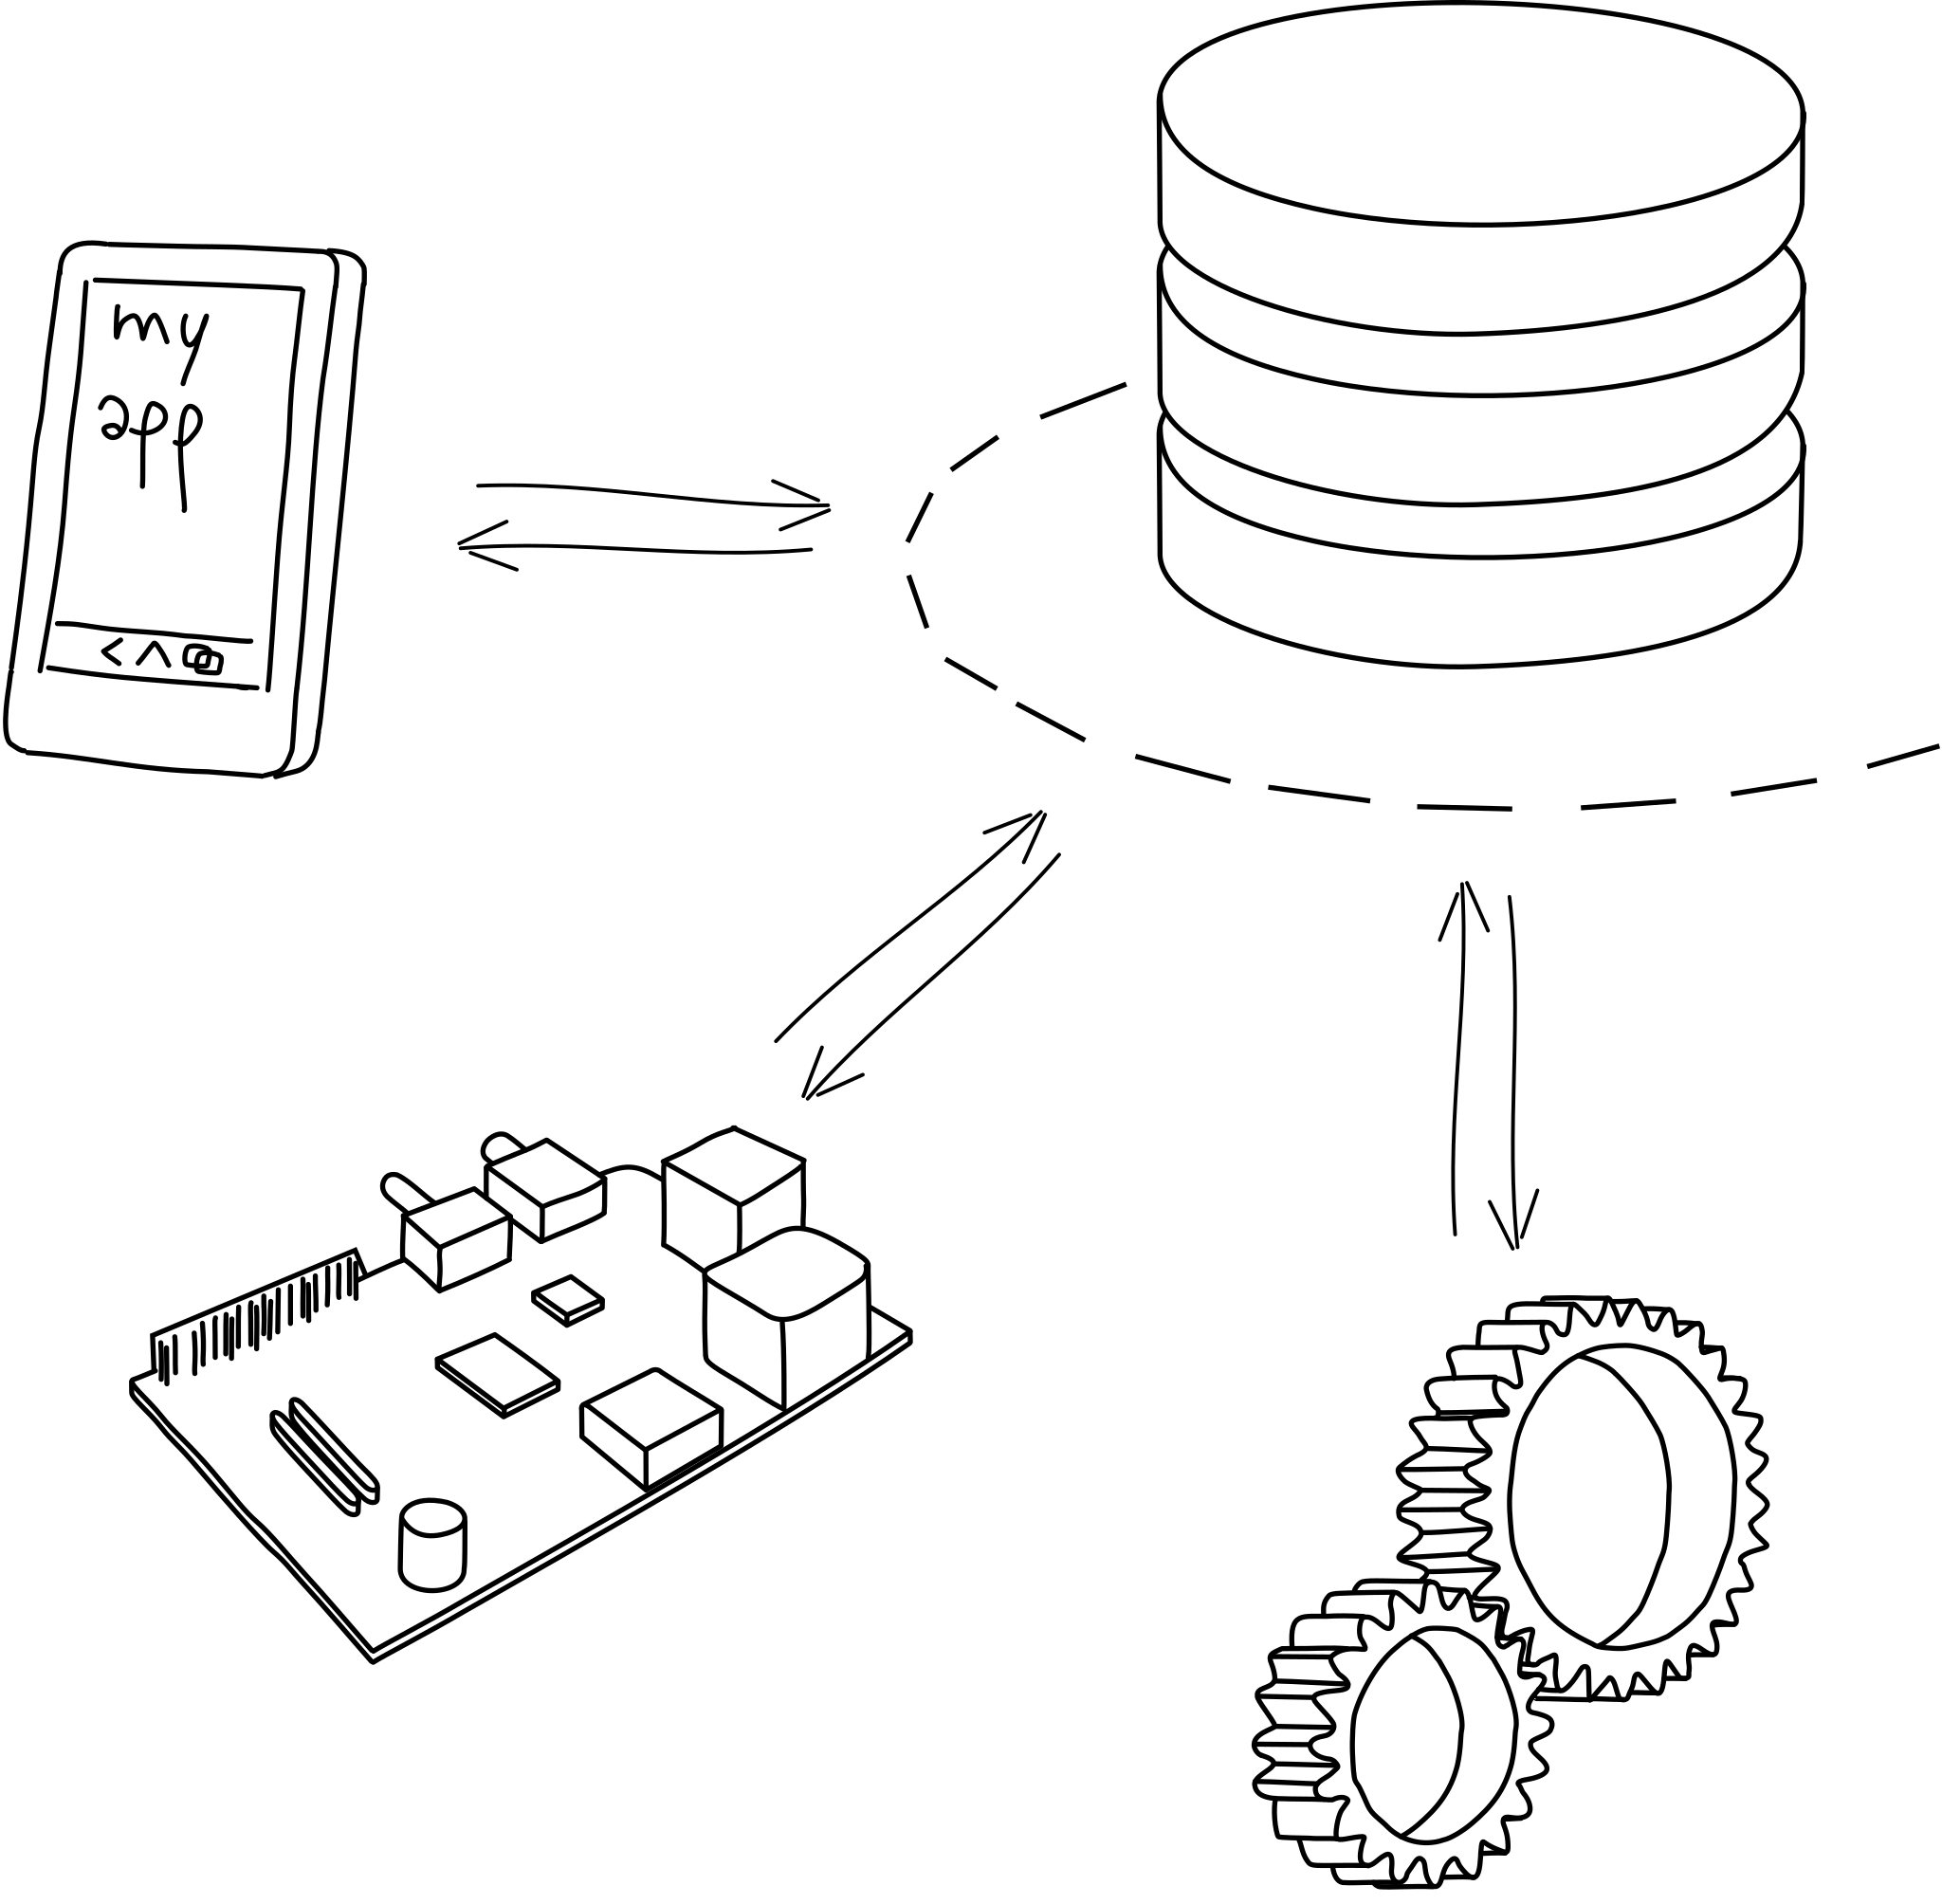
\includegraphics[width=0.24\textwidth]{img/IoT.pdf}
                \begin{center}
                \begin{scriptsize}
                    Les communications directes et bidirectionnelles permettent de développer facilement des applications multi-composants.
                    % (communications directes et bidirectionnelles) 
                \end{scriptsize}
                \end{center}
            \end{wrapfigure}
            
        
            Les développements reposent pour beaucoup sur les connaissances et l'expertise que l'équipe a accumulées pendant plus de dix ans dans le contexte de la recherche sur le calcul distribué haute performance, au sein notamment du laboratoire LMT-Cachan. Certains des développements ont par ailleurs été réalisés en prenant comme base des idées publiées par des équipes de l'INRIA, avec lesquelles des partenariats sont en cours.

            \medskip
            L'approche a été validée avec succès sur plusieurs types d'applications, impliquant des développeurs de provenances diverses. La première version a permis de \textbf{confirmer les gains attendus en terme de temps de développement} pour des interfaces pour le calcul et la visualisation scientifique, des applications web collaboratives et des systèmes de contrôle de machines physiques. Suite à cette première version, un travail important est réalisé sur l'extensibilité et l'optimisation des protocoles et des implémentations, conduisant à des \textbf{gains significatifs concernant l'utilisation des espaces de stockage, des processeurs et de la bande passante}, tout en garantissant la meilleure expérience utilisateur.
            

    % ----------------------------------------------------------------------------------------------------------------------------
    \section{Description du produit, service ou procédé}

        SocaDB est un Système de Gestion de Base de Données (SGBD), au même titre par exemple MongoDB, Couchbase, MySQL, ... SocaDB permet donc de stocker des données, puis de les retrouver selon différents critères. De la même manière que MongoDB ou Couchbase, SocaDB propose aussi des solution aux problèmes d'échelles et de résilience que posent les configuration cloud de plus en plus courantes.
        
        SocaDB se démarque par le fait qu'il a été conçu pour \textbf{simplifier et accélérer de façon considérable le développement des applications connectées}, tout \textbf{en garantissant le meilleur usage des ressources}.
        
        %         Du point de vue de l'utilisateur, SocaDB offre les mêmes fonctionnalités de bases qu'un système de fichier
                
        %         SocaDB offre les mêmes fonctions basiques qu'un système de fichiers mais en permettant une bien plus importante mutualisation des moyens, avec un niveau de fonctionnalité sensiblement plus élevé.
        
        %         Il s'agit d'un . La réactivité et la gestion des droits permettent basiquement de simplifier et accélérer de façon extrêmement importante le développement d'applications impliquant en parallèle différents objets, algorithmes et/ou utilisateurs.
    
        %         SocaDB prend en interne la charge de la gestion fine des règles et des droits de collaborations.
    
        %         Les protocoles de communication, permettant d'adresser de façon bidirectionnelle toutes les cibles supportant les communications internet (applications web, bureau, embarqué ou mobile), sont conçus pour exploiter au mieux les ressources informatiques.

        %         SocaDB a vocation à gérer les données et la communication des applications informatiques connectées. De prime abord, comme toutes les bases de données, SocaDB permet de stocker et retrouver des données, de volume arbitrairement grand, en répondant aux problèmes de résilience et d'extensibilité. Il est possible en outre de suivre et de \textit{contrôler} des évolutions de données variées et potentiellement complexes, à l'aide d'un modèle de programmation qui conduit à simplifier et accélérer de façon extrême le développement d'une grande variété d'applications.
        
        En pratique, et pour rentrer plus dans les détails techniques, SocaDB propose d'éliminer les intersticiels (middlewares) : les applications (côté client ou côté serveur) se connectent \textbf{directement} à la base de données, établissant (de façon optionnelle) une communication \textbf{bi-directionnelle}. Les droits, la surveillance, les modifications parallèles et le lien avec les programmes de service sont donc gérés au niveau même de la base de données. Ces propriétés permettent d'accéder à des niveaux \textbf{de facilité, de cohérence, de sécurité et de résilience} sensiblement plus élevés qu'avec ce qui serait possible d'obtenir en codant les différentes logiques dans des intersticiels spécifiques (à coder et assembler pour chaque projet, comme pratiqué de façon usuelle).
        
    % ----------------------------------------------------------------------------------------------------------------------------
    \section{Caractère innovant de la technologie}
                
        \subsection{Rapidité de développement}

            % Il convient en outre de considérer
        
            % Le premier contact avec un système doit nécessairement de nos jours être le plus doux possible, sous peine de ne pas être considéré par la plus grand masse des développeurs utilisateurs. Sauf très rares exceptions (dans le cas industriel par exemple) les bases de données actuelles présentent donc toutes des chemins d'accès évidents. SocaDB ne fait pas exception à la règle.

            \begin{wrapfigure}{r}{0.25\textwidth}
                \hfill
                \vspace{-1.2em}
                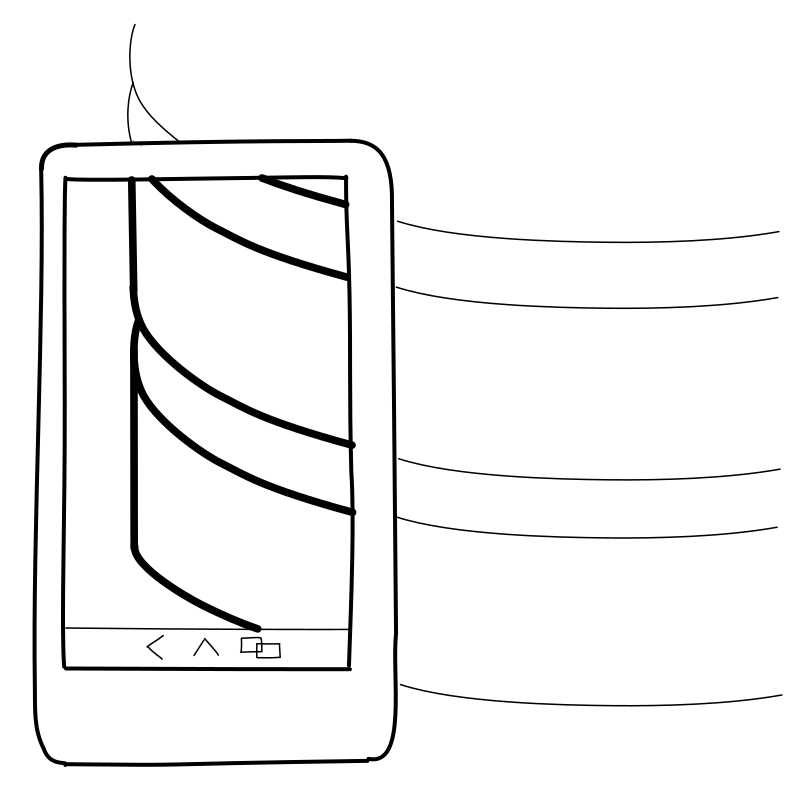
\includegraphics[width=0.25\textwidth]{img/DD_view.pdf}
                \begin{center}
                \begin{scriptsize}
                    Côté client, SocaDB fonctionne comme un ``cache'' d'utilisation transparente. Les applications ont accès à la puissance du cloud, à la vitesse du local.
                    % (communications directes et bidirectionnelles) 
                \end{scriptsize}
                \end{center}
            \end{wrapfigure}

            Concernant les bases de données actuelles, sauf très rares exceptions, les premiers contacts sont toujours très agréables. Les premiers exemples tiennent en quelques lignes. Mais sorti des applications triviales, ces modèles de programmation très simples à expliquer parce que rudimentaires, mènent à une complexité prohibitive : comment par exemple gérer efficacement les indirections, les hétérogénéités de données et de comportements, la synchronisation, les flux, les modifications en parallèles des mêmes jeux de données, ... ?
            
            % En permettant aux utilisateurs de définir de nouveaux types, en gérant les pointeurs et les aspects hiérarchiques.
            
            Dans le but d'aider les développeurs de développer simplement de applications complexes, SocaDB permet en particulier de \textbf{typer leurs données}, en utilisant des définitions déjà existantes, ou en proposant leurs propres définitions et en y associant leurs méthodes. Les méthode concernent spécifiquement la synchronisation, la compression, les requêtes, l'exploration de pointeurs, etc... c'est à dire l'interaction avec la base de donnée (il ne s'agit pas de méthodes distribuées comme dans les bases de données orientées objet). Cette information permet à SocaDB d'\textbf{assister les développeur sur un bien plus grand nombre de taches} que si les données n'arrivaient exclusivement que sous forme d'agrégats de types primitifs (comme avec du JSON ou même du SQL par exemple). % Ceci permet en particulier, de gérer de façon beaucoup plus efficace les données d'applications complexes qui peuvent impliquer une grande variété de types écrits avec des motifs de conception associés à une grande variété de besoins (pointeurs, compacité, héritage, ...).
            
            \medskip
            Par ailleurs, les clients (les composants d'une application) peuvent de façon optionnelle de \textbf{connecter de façon bidirectionnelle} à la base de donnée (via websocket ou ssl directement). Ceci permet simplement et efficacement à SocaDB d'agir de façon pro-active et de prendre en charge la synchronisation, les flux, les événements, ... éliminant le besoin de couches supplémentaires pour assurer ces taches.
            
            En outre, SocaDB propose aux clients de fonctionner comme un ``cache'' : les clients fonctionnent via des \textbf{serveurs locaux}, pouvant stocker de façon temporaire ou permanente (c'est à dire en RAM et sur disque dur si disponible) des copies locales des valeurs les plus utilisées. Ces copies sont synchronisées de façon automatique : les clients sont immédiatement informés des modifications effectuées par des tiers (autre utilisateur, objet ou programme de service) et quand un client modifie une donnée, la modification est automatiquement envoyée au serveur. Ceci élimine notamment le besoin de gérer soit même les requêtes AJAX pour les applications Web, et \textbf{ajoute de façon automatique la fonctionnalité ``off-line''} (possibilité de travailler en absence de connexion).

        \subsection{Sécurité}
        
            La quasi-totalité des base de données actuelles ne proposent des modèles de sécurité qu'à des granularités très grossières. Les bases de données SQL par exemple ne gèrent les droits qu'au niveau des tables. Sauf rares exceptions, les dévelop\-peurs se retrouvent donc systématiquement en charge de coder leur propre logique de sécurité, et en général dispersé dans de multiples couches.
            
            En plus de faire perdre un temps significatif, ce mode de fonctionnement augmente considérablement le risque de failles de sécurité. La logique de sécurité se retrouve disséminée, rendant plus ardus la compréhension et le contrôle (cf. par exemple les failles récurrentes des applications WordPress pour ne citer qu'elles).
            
            \medskip
            \textbf{SocaDB propose a contrario de gérer la sécurité en interne}, en prenant en charge l'authentification, les droits et le contrôle d'accès. Le niveau de granularité et choisi par le développeur.
            
        \subsection{Flexibilité}

            On ne compresse ni ne modifie de la même manière une image de grande taille ou du texte littéraire. De même on ne va pas y faire les mêmes genres de requêtes, etc... Ces types de données pouvant cohabiter au sein des données d'une même application, on s'attend à ce que les bases de données permettent de gérer cette forme d'hétérogénéité. Pourtant, sorti des quelques types rudimentaires, la quasi totalité des système actuels ne proposent qu'un seul mode de fonctionnement pour tous les types d'opérations, et quelque soit les type de donnée. En pratique les bases de données conventionnelles conduisent dans le meilleur des cas à des assemblages complexes dès lors que plusieurs cas d'utilisation sont présents (par exemple on utilisera TempoDB pour les données capteurs, MySQL pour les données clients, etc...). Dans le pire des cas qui arrive malheureusement assez souvent, les systèmes, même spécialisés, sont conçus en dur avec des hypothèses qui ne collent pas aux besoins.
        
            \medskip
            En définissant leurs types de données les développeurs peuvent dans SocaDB associer un certain nombre de méthodes de gestion (par exemple concernant la compression, le suivi, les modifications, la gestion des droits, les requêtes, ...). Cette possibilité permet de façon naturelle de faire \textbf{cohabiter une grande variété de besoins} -- dont certains ne sont du reste pas couverts par aucun système actuel -- dans un espace de nom homogène, et en optimisant les ressources.
            
        \subsection{Collaboratif temps-réel}

            \begin{wrapfigure}{r}{0.3\textwidth}
                \hfill
                \vspace{-1.2em}
                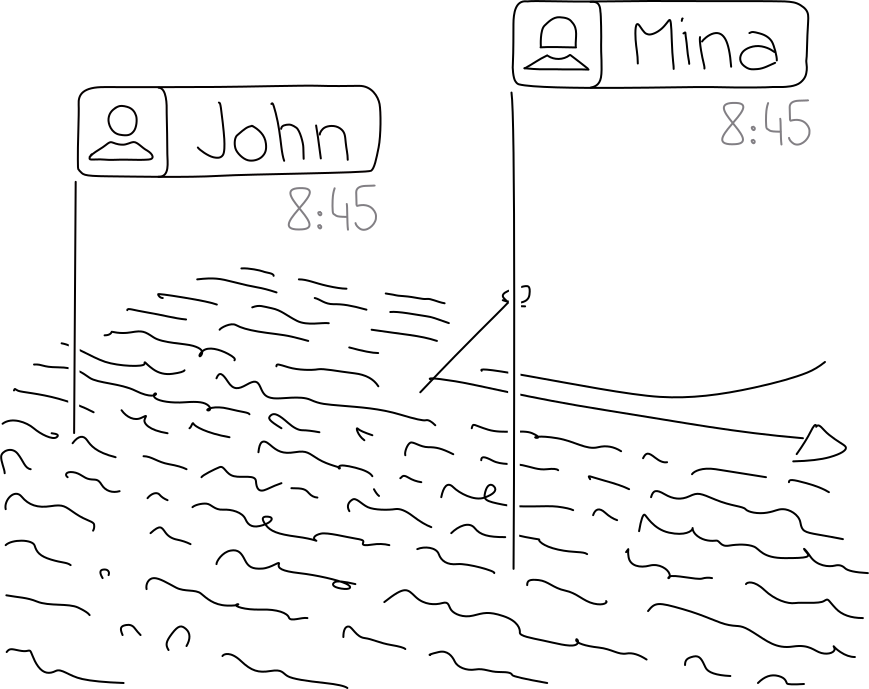
\includegraphics[width=0.3\textwidth]{img/sharing.pdf}
                \begin{center}
                \begin{scriptsize}
                    SocaDB permet de définir des règles de collaboration, permettant de gérer de façon effective la modification en parallèle des mêmes jeux de données, quels que soient leurs types.
                \end{scriptsize}
                \end{center}
            \end{wrapfigure}

            Si plusieurs utilisateurs modifient en parallèle le même jeu de données (par exemple le même texte ou la même image, au même paragraphe, dans la même zone ou non), les bases de données actuelles se contentent d'écraser les modifications reçues en premier. Sans outils supplémentaires, les systèmes actuelles ne permettent donc pas de collaboration temps-réel sur les données qui y sont stockées.
            
            La parade actuelle consiste a ajouter une couche de ``transformation opérationnelle'' au niveau des clients, mais qui est extrêmement complexe à implémenter, et souvent inefficace au niveau du temps d'exécution.
            
            \medskip
            SocaDB propose quand à implémente la ``synchronisation différentielle'' au sein même de la base de données, et ce pour des types quelconques, non limités à des combinaisons simples de types primitifs. En plus de permettre de façon extrêmement simple de \textbf{développer des applications collaboratives temps-réel}, cette gestion en interne permet de rendre le \textbf{modèle de sécurité plus puissant et plus précis} (on peut par exemple n'autoriser que certains types de modifications pour certains utilisateurs) et de parvenir à une bien meilleure exploitation des ressources (on n'envoie que les changements, ce qui peut avoir une grande importance pour les objet de volume important).
            
            % Ce fonctionnement permet aussi de proposer une façon simple de rendre collaboratives des applications qui n'y étaient pas destinées.

            
        \subsection{Performance}
        
            La recherche de performance a pour volonté d'améliorer l'expérience utilisateur, mais aussi de \textbf{minimiser la consommation de ressources} (temps CPU, taille et nombre des supports de stockage, ...) à l'origine de coûts écologiques et économiques qui peuvent devenir très importants.
        
            \medskip
            SocaDB est conçu pour être performant. C'est bien sûr valable pour l'implémentation, mais contrairement aux autres systèmes, \textbf{SocaDB le fait en fonction de l'ensemble du système}, agissant en particulier sur les protocoles. Un travail sur la compacité des représentations, le typage, la minimisation du nombre de requêtes et d'intermédiaires sont notamment à l'origine de gains significatifs au niveau bande passante, utilisation CPU, utilisation RAM et disques durs.

    % ----------------------------------------------------------------------------------------------------------------------------
    \section{Liberté d’exploitation, éventuels risques de contrefaçon}

        \subsection{Limitations d'usage}
        
            SocaDB est un logiciel libre (licence LGPLv3), développé hors de tout contexte professionnel (cf. en annexe le document signé par le directeur du laboratoire d'origine du porteur de projet, spécifiant que le développement dont il est question ne faisait pas partie des missions lorsque le porteur de projet en était salarié).
        
            À la connaissance des auteurs, aucun brevet n'est à même d'en limiter l'usage, mais l'analyse devra impérativement être poussée plus avant par un cabinet spécialisé : les premières recherches n'ont été effectuées que par le porteur de projet seul, sans compétences particulières dans le domaine.
        
            \medskip
            %Le logiciel n'utilise que très peu de librairies et donc n'utilise que très peu d'outils à même de limiter l'usage.
            Les librairies utilisées par SocaDB sont~:
            \begin{itemize}
                \item Celo (\verb&https://github.com/hleclerc/Celo&), sous licence LGPLv3 (maintenue par le porteur de projet)
                \item PrepArg (\verb&https://github.com/hleclerc/PrepArg&), sous licence LGPLv3 (maintenue par le porteur de projet)
                \item OpenSSL (\verb&https://www.openssl.org&), sous licence Apache 1.0, de type BSD.
            \end{itemize}
        
        \subsection{Brevetabilité}

            L'idée de mettre la base de données en accès frontal est clairement une façon de limiter les besoins en matériel informatique. Bien qu'on en trouve les prémisses dans Firebase, l'idée n'est absolument pas répandue et semble nouvelle. Des premières recherches de la part du porteur de projet n'ont pas permis de trouver de brevets sur cette idée. Un cabinet spécialisé permettra de valider l'hypothèse et vraisemblablement d'organiser le dépôt d'un brevet.
        
        \subsection{Risques de contrefaçon}
        
            Il est important de signaler que dans le domaine du logiciel, la rapidité d'exécution compte souvent plus que l'idée elle-même. Poussés par le \textbf{time-to-market}, les grands acteurs se retrouvent souvent à racheter des entreprises n'ayant pourtant produit que des logiciels libres, autour d'idées publiques et faits avec un nombre limité de lignes de codes... ce qui prouve que bien que la contrefaçon soit parfois accessible, c'est rarement la solution retenue.
            
            Il faut ajouter que le domaine des bases de données est spécialisé, demandant des compétences très particulières (en optimisation, parallélisme, gestion de E/S, ...), ce qui est à même de décourager la contrefaçon.
            
            \medskip
            Du reste, l'objectif de la structure envisagée ne sera jamais de vendre le produit en tant que tel, mais plutôt l'expertise qui va autour.

    % ----------------------------------------------------------------------------------------------------------------------------
    \section{Aspects réglementaires}

        Le marché des bases de données est effectivement très réglementé, surveillé notamment par la CNIL, mais SocaDB n'est pas une base de données, c'en est uniquement un système de gestion. L'essentiel des responsabilités décrites par la CNIL reposera donc sur les clients, ou pour être plus précis sur les clients des développeurs qui utiliseront SocaDB.
        
        Pour le sujet de réglementations liées aux bases de données, le but de SocaDB sera essentiellement de \textbf{permettre à ses clients de respecter leurs responsabilités}. En pratique le seul point qui peut poser question est celui de la sécurité. Les pré-requis sont tous extrêmement basiques, sauf potentiellement pour ce qui concerne les questions de sécurité : SocaDB pourrait être tenu fautif d'un manque d'étanchéité en cas de présence de failles de sécurité. Un \textbf{audit de sécurité} est donc prévu pour minimiser ce risque.
        
        \medskip
        Pour être complet il faut néanmoins ajouter que SocaDB ne sera pas le seul produit proposé. Il est notamment prévu de proposer SocaDB en DBaaS (DataBase as a Service) c'est à dire de \textbf{vendre du stockage et du temps de machines contenant des instances de SocaDB}. Les exemples de Firebase ou de Mongolab pourront servir de modèle pour les aspects réglementaires, mais au vu de la complexité du sujet, le passage pas un cabinet d'avocat est inévitable.
        
    % ----------------------------------------------------------------------------------------------------------------------------
    \section{Études de faisabilité technique réalisées}

        Un premier prototype a permis de valider le modèle de programmation. Une version beta a ensuite permis de valider les choix techniques, montrant la possibilité de fonctionner de façon extensible, sûre, avec des vitesses d'exécution et des utilisations de ressources largement compatibles avec les objectifs annoncés.

        Les premiers retours de développeurs sont tous très positifs, avec néanmoins quelques affinages à prévoir au niveau des interfaces de programmation.
        
        Le développement de la première version publique sera donc assez cadrée, et sera réalisée dans des temps raisonnables.
        
% --------------------------------------------------------------------------------------------------------------------------------
% --------------------------------------------------------------------------------------------------------------------------------
% --------------------------------------------------------------------------------------------------------------------------------
\chapter{Équipe}

    % ----------------------------------------------------------------------------------------------------------------------------
    \section{Fonctions et contributions du candidat et des membres de l’équipe}
    
        
        Discussions en cours :
        \begin{itemize}
            \item Hugo Leclerc (porteur de projet) : se chargera de la présidence et de l'architecture du projet.
            \item Gainant Gérald : directeur technique ?
            \item Cédric Coursin : directeur général + responsabilités commerciales (essentiel notamment pour le démarrage en mode SSII)
        \end{itemize}

        \medskip
        Par ailleurs, le comité stratégique tel que défini actuellement contient
        \begin{itemize}
            \item Jérémie Bellec, président de structure-computation, développement d'applications SaaS complexes
            \item Discussions en cours pour une personne du board de GMC, développement de logiciels pour communication client.
            \item Une personne du board de Stample (se mettre d'accord la dessus), solution internet pour favoriser la collaboration.
            \item Discussions en cours auprès de développeurs ou utilisateurs de bases de données de la communauté du logiciel libre.
        \end{itemize}
    
    % ----------------------------------------------------------------------------------------------------------------------------
    \section{Compétences et expériences professionnelles du candidat et des membres de l’équipe}
    
        Je suis passionné de programmation depuis mon plus jeune âge. Nous pourrons noter :
        \begin{itemize}
            \item la participation à un groupe de ``demomaker'' 
                \begin{itemize}
                    \item[$\rightarrow$] acquisition dès le collège de compétences fortes en développement optimisé pour la vitesse d'exécution et l'occupation mémoire
                    \item[$\rightarrow$] deuxième place d'un concours national de création de logiciel (Soft Qui Peut).
                \end{itemize}
                
            \item Une thèse en mécanique et mathématiques appliquées
                \begin{itemize}
                    \item[$\rightarrow$] premier contact avec le domaine des ``data sciences''
                \end{itemize}
            
            \item Un poste d'ingénieur de recherche au sein du LMT-Cachan (au sein de l'ENS-Cachan, pendant 10 ans)
                \begin{itemize}
                    \item[$\rightarrow$] utilisation et de participations au développement de connaissances dans le domaine du HPC (calcul haute performance), impliquant le parallélisme, de calculs et du stockage de grand taille, et pour des besoins variés.
                \end{itemize}
            
        \end{itemize}

        Autre personnes à compléter si accord.
        \begin{itemize}
            \item Gainant Gérald : Senior Generalist Lo/Hi Level and Graphics Programmer on Realtime platforms, SW Designer and Architect, Entrepreneur. 
            \item Cédric Coursin : Responsable marketing BMW.
            \item ...
        \end{itemize}

    
    % ----------------------------------------------------------------------------------------------------------------------------
    \section{Motivation, engagement personnel du candidat}
        %Pour les candidats salariés, joindre un accord de l’employeur sur le projet présenté
        
        Pour mener à bien sa mission, le candidat quitte son poste du CNRS à partir du ...
        
    % ----------------------------------------------------------------------------------------------------------------------------
    \section{Recrutements prévus}

        Nous aurons besoin d'un développeur très compétent en javascript/html5 sera assez vite nécessaire pour la création en mode SSII de sites internet, pour les interfaces d'administration et l'interfaçage des librairies web les plus utilisées par la communauté (emberjs, angularjs, ...). Pour ce poste, des discussions sont en cours avec Timotée Neullas, ingénieur IMAC, travaillant actuellement chez Sony en CDD (à 40k\texteuro{} net par an). Il sera disponible au second semestre 2015.

        À moyen terme, pour les contrats de maintenance et les développements ad-hoc, nous aurons besoin de développeurs C++. Ce genre de profil est difficile à trouver. Nous cherchons pro-activement via la recherche en informatique et le développement de jeux vidéos. Par ailleurs, SocaDB étant libre, nous faisons en sorte d'ouvrir la porte à toutes les volontés de contribution, augmentant nos chances de trouver des développeurs intéressés et compétents.
        
% --------------------------------------------------------------------------------------------------------------------------------
% --------------------------------------------------------------------------------------------------------------------------------
% --------------------------------------------------------------------------------------------------------------------------------
\chapter{Marché visé}

    \section{Modèle d'affaires}
    
    % PARLER DE LA MÉCANIQUE DU DÉBUT.
    % Pourquoi on sera meilleurs qu’eux sur le marché du début (sites collaboratifs).
    
    Le modèle d'affaires retenu est en substance le même que celui des entreprises derrières MongoDB et CouchBase. Ces entreprises font respectivement 62M\$ et 80M\$ de chiffre d'affaire, en étant valorisées à 1.2B\$ et 950M\$, ce qui prouve la viabilité de leur modèle économique.
    
    Leur produit de base est open-source. Ce fonctionnement permet de réduire de façon significative les coûts de communication et d'acquisition client. Il s'agit du reste d'un standard de fait, peu de développeurs dans les cibles visées étant disposés à payer pour un logiciel de ce genre. Néanmoins, le logiciel ne fait pas tout : \textbf{il est difficile de maîtriser complètement le produit sans une aide importante}.
    
    \medskip
    Au sein d'une entreprise, les données sont considérées comme un capital important. Une entreprise ne peut donc pas se permettre de laisser des zones d'ombre et du hasard concernant l'utilisation et la gestion des bases de données. Beaucoup d'entreprises ont donc intérêt à faire appel à de l'expertise, les développeur du produit étant clairement les plus pertinents pour cette tache.

    Ceci se traduit pour les clients en besoin
    \begin{itemize}
        \item de formation (sur site, ou dans des conférences)
        \item de développement pour des besoins spécifiques (ex: types d'objets à stocker, ...)
        \item de contrats de maintenance (engagement sur le délai des réponses, maintenance sur site, ...)
    \end{itemize}

    À moyen et long terme, il est donc prévu de vendre essentiellement de l'expertise, le produit principal étant gratuit.
    
    \medskip
    Néanmoins, ce mode de fonctionnement ne permet pas seul de créer un démarrage dans les meilleures conditions. L'expérience montre qu'il faut compter un minimum de deux à trois ans pour un premier retour avec ce genre de modèle.
    
    Une première solution pourrait consister à chercher des financements importants dès le début (par exemple comme pour MeteorJS ou TempoDB ou en fait, bon nombre d'autres entreprises américaines), mais il sera très important d'être en mesure de montrer très vite la viabilité du produit sur des exemples réels.
    
    La proposition est donc de démarrer assez sur le principe d'une SSII pour la création de sites internet (démonstratifs), permettant d'assurer une première source de revenu.
    
    %    En outre, afin de favoriser l'adoption de la technologie, nous chercherons au début à proposer nos services pour la création d'applications multi-composants et/ou avec des besoins de collaboratif temps réel (via le web ou non). Le but est de créer des applications pour mettre en avant les capacités de SocaDB, en récoltant autant que faire ce peux des premières ressources. Compte tenu du modèle choisi, le retour sur SocaDB en tant que tel a en effet peu de chance de devenir significatif plusieurs années d'activité.

    \medskip
    Le modèle d'affaire est synthétisé dans le tableau suivant~:
    
    % \hspace{-0.34\textwidth}
    \begin{sideways}
    \begin{small}
    \begin{minipage}{\textheight}
     
    \hrulefill \medskip
    
    \begin{minipage}[t]{0.19\textheight}
    \begin{flushleft}
        \textbf{\color{MSBlue}\large Key partners}\\
        $\bullet$~Developers working on the SocaDB ecosystem (libraries or tools based on SocaDB)\\
        $\bullet$~Community (developers sharing or pointing out their expertise on SocaDB)
    \end{flushleft}
    \end{minipage}
    \hfill
    \begin{minipage}[t]{0.19\textheight}
        \begin{minipage}[t]{\textwidth}
        \begin{flushleft}
            \textbf{\color{MSBlue}\large Key activities}\\
            $\bullet$~Increase the performances of SODA and derivatives.(speed latency, simplicity)\\
            $\bullet$~Growth of the ecosystem\\
            $\bullet$~Custom developments\\
            $\bullet$~Expertise\\
            $\bullet$~Training
        \end{flushleft}
        \end{minipage}
        
        \vspace{1.0em} \hrulefill \medskip
        
        \begin{minipage}[t]{\textwidth}
        \begin{flushleft}
            \textbf{\color{MSBlue}\large Key resources}\\
            $\bullet$~Developers with\\
            ~$\circ$~high expertise on the product\\
            ~$\circ$~high expertise on high performance programming\\
            $\bullet$~UI developers and graphic designers\\
            $\bullet$~Administrators for installation
        \end{flushleft}
        \end{minipage}
    \end{minipage}
    \hfill
    \begin{minipage}[t]{0.19\textheight}
    \begin{flushleft}
        \textbf{\color{MSBlue}\large Value proposition}\\
        Extreme simplification of the development of efficient connected web, desktop or mobile applications\\
        $\bullet$~straightforward synchronization primitives\\
        $\bullet$~automatic collision management for parallel modifications on the same data\\
        $\bullet$~straightforward management of security and authentication\\
        $\bullet$~interoperability (C++, javascript, web, desktop or mobile, \dots)\\
        $\bullet$~efficient and automatic caching, compression\\
        $\bullet$~24/365, automatic failure and scaling management
    \end{flushleft}
    \end{minipage}
    \hfill
    \begin{minipage}[t]{0.19\textheight}
        \begin{minipage}[t]{\textwidth}
        \begin{flushleft}
            \textbf{\color{MSBlue}\large Customer relationship}\\
            $\bullet$~Dedicated personal assistance (on-site, forums, phone, mail, …)\\
            $\bullet$~Conferences, training sessions\\
            $\bullet$~Documentation, blogs, forums, ...
        \end{flushleft}
        \end{minipage}
        
        \vspace{3.5em} \hrulefill \medskip

        \begin{minipage}[t]{\textwidth}
        \begin{flushleft}
            \textbf{\color{MSBlue}\large Channels}\\
            $\bullet$~Ext. blogs, forums and conferences\\
            $\bullet$~Web site, mailing, RSS\\
            $\bullet$~Self hosted conferences
        \end{flushleft}
        \end{minipage}
    \end{minipage}
    \hfill
    \begin{minipage}[t]{0.19\textheight}
    \begin{flushleft}
        \textbf{\color{MSBlue}\large Customer segments}\\
        $\bullet$~Developers (individual or from companies) of any kind of connected applications, collaborative or not, desktop, web or mobile\\
        $\bullet$~Companies relying on SocaDB for storage or the data of their customers
    \end{flushleft}
    \end{minipage}

    \vspace{1em} \hrulefill \medskip

    \begin{minipage}[t]{0.49\textheight}
    \begin{flushleft}
        \textbf{\color{MSBlue}\large Cost structure}\\
        $\bullet$~Value driven for the development of the main product\\
        $\bullet$~Cost-driven for service contracts and ad-hoc developments (internal resources), formations/conferences (room renting, …)\\
        $\bullet$~Customer support\\
        $\bullet$~Customer care
    \end{flushleft}
    \end{minipage}
    \hfill
    \begin{minipage}[t]{0.49\textheight}
    \begin{flushleft}
        \textbf{\color{MSBlue}\large Revenue streams}\\
        $\bullet$~Subscription fees from the service contracts\\
        $\bullet$~Licensing of the “professional editions”\\
        $\bullet$~Registrations for formations and conferences\\
        $\bullet$~Revenues from expertise and ad-hoc development
    \end{flushleft}
    \end{minipage}

    \vspace{1em} \hrulefill

    \begin{center}
        \footnotesize
        \bigskip
        \textit{Business Model Canvas} de l'activité
    \end{center}


    \end{minipage}
    \end{small}
    %     \end{rotate}
    
    \end{sideways}
    
    
    
    % ----------------------------------------------------------------------------------------------------------------------------
    \section{Informations sur la concurrence}
    
        La problématique très générale de la gestion de données est traitée par un nombre considérable de produits.
    
        Si nous nous concentrons plus spécifiquement sur ceux qui sont susceptible d'être utilisés pour les applications ciblées, nous pourrons citer~:

        \begin{enumerate}
            \item Firebase (\verb&https://www.firebase.com/&) qui est un service permettant de stocker, lire et surveiller des données au format JSON. En terme de modèle de programmation, c'est le produit le plus proche de SocaDB. L'entreprise a été rachetée par Google en septembre 2014.
            \item Google Drive API (\verb&https://developers.google.com/drive/&) est une interface de programmation permettant à des programmes de stocker, lire et surveiller des données au format JSON, comme firebase, mais avec une gestion des modifications parallèles (par synchronisation différentielle). Dans ce cas, ce sont les utilisateurs qui sont responsables de leur données et de leur coût de maintien (cession des données personnelles et/ou abonnements Google for work). Firebase quand à elle fait reposer ce coût sur les éditeurs des logiciels.
            \item MongoDB (\verb&https://www.mongodb.org&) est une base de données NoSQL open-source. Elle permet de stocker et lire des données au format JSON. Les développeurs peuvent l'installer eux même, et doivent nécessairement l'utiliser à travers un middleware, avec du code à écrire pour chaque projet pour la logique de sécurité, l'interfaçage avec les codes exécutés sur les clients, \dots Le traitement analytique est permis par un système du type ``map-reduce''.
            \item Couchbase (\verb&https://www.couchbase.com&) fonctionne sur le même principe que MongoDB, avec une interface très similaire. Couchbase se positionne comme étant plus rapide et plus facilement ``scalable'' que MongoDB.
            \item MySQL et ses variantes (très nombreuses) proposent de stocker les données sous forme de tableau, et l'accès se fait via un langage qui fait référence (étudié notamment dans les écoles d'informatique). Parmi ses variantes, certaines prétendent proposer une très bonne extensibilité, avec de très bonnes vitesses d'exécution (ex : FoundationDB).
            \item MeteorJS (\verb&https://www.meteor.com&) est un middleware qui permet à une application javascript d'être informée en temps-réel des modifications sur des données stockées dans des bases de données conventionnelles (pour l'instant uniquement MongoDB). MeteorJS gère aussi l'exécution de code javascript côté serveur.
            \item Connext DDS (\verb&https://www.rti.com&) est un système de messagerie industriel, pour la communication efficace entre entités. Connext DDS supporte la persistance des données, de sorte qu'il est légitime de le considérer comme un système de gestion de données.
            \item Intersystems (\verb&http://www.intersystems.com/fr/&) propose le même genre de fonctionnalités que Connext DDS, avec un ciblage différent (centré sur le secteur de la santé).
        \end{enumerate}

        % Au niveau du modèle de programmation proposé, Firebase est le concurrent le plus proche. Comme expliqué au chapitre suivant, le positionnement est par contre très différent, se traduisant par des choix techniques différents (API et implémentations) et des marchés se recouvrant peu.
        
    % ----------------------------------------------------------------------------------------------------------------------------
    \section{Avantages concurrentiels}

        Parmi les solutions citées pour stocker transmettre et retrouver des données, très peu voire aucune n'a été conçue \textit{directement} pour les marchés visés par SocaDB (applications interactives, potentiellement multi-composant, potentiellement collaboratives et potentiellement complexes). En pratique, les bases de données ne proposent aujourd'hui qu'un niveau de service rudimentaire, impliquant la nécessité d'ajouter une quantité considérable de couches complexes, à revoir à chaque nouveau projet, pour arriver aux fonctionnalités requises.
        
        Le premier argument, celui qui poussera les développeurs à tester puis à utiliser SocaDB, c'est donc la \textbf{vitesse de développement}. Cette dernière inclue incluant la vitesse d'apprentissage, d'installation et de développement, que ça soit pour les \textbf{applications simples ou complexes}.
        
        \medskip
        Par ailleurs, l'intégration de fonctionnalités importantes dans le c\oe{}ur de la base de données conduit à des gains significatifs concernant les temps de réponse et l'utilisation des ressources.
        
        Au delà des gains concernant l'expérience utilisateur, ce saut quantitatif permet d'\textbf{adresser des marchés peu ou actuellement mal couverts par les bases de données}. L'IoT soulève par exemple des problèmes de gestion d'événements, de synchronisation, de fonctionnement distribué (multi-composant) et d'économie de ressources. SocaDB y apportera justement des réponses déterminantes.
        
        \medskip
        La figure suivante permet de représenter de façon synthétique la position par rapport à la concurrence. Les items sont détaillés plus bas.
        
        \begin{center}
        \begin{tikzpicture}
            \begin{axis}[
                    width = \textwidth,
                    height = 0.5\textwidth,
                    font = \footnotesize,
                    ymin = -0.1,
                    ymax = 1.1,
                    xtick = { 0, 1, 2, ..., 9 },
                    ytick = { 0, 1 },
                    x tick label style = { rotate = 45, anchor = east, yshift = -0.5\baselineskip },
                    legend style = {
                        at={(0.46,1.03)},
                        anchor=south
                    },
                    % transpose legend,
                    legend columns = -1,
                    xticklabels = {
                        Collaboration temps-réel,
                        Données complexes,
                        Flexibilité,
                        Modèle de sécurité,
                        Traitements analytiques,
                        Interfaçages potentiels,
                        Gestion des ressources,
                        Confiance dans l'entreprise,
                        Simplicité du 1\up{er} tutoriel,
                    },
                    yticklabels = { Bas, Haut },
                ]

                \addlegendentry{\tiny{Firebase/Google}}
                \addplot[ blue, mark = triangle ] coordinates { %M, dashdotdotted
                    ( 0, 0.8 )  % Collaboration temps-réel,
                    ( 1, 0.15 ) % Données complexes,
                    ( 2, 0.1 )  % Flexibilité,
                    ( 3, 0.5 )  % Modèle de sécurité,
                    ( 4, 0.0 )  % Traitements analytiques,
                    ( 5, 0.5 )  % Interfaçages potentiels,
                    ( 6, 0.0 )  % Gestion des ressources,
                    ( 7, 0.2 )  % Confiance dans l'entreprise,
                    ( 8, 1.0 )  % Simplicité 1er tutoriel,
                };
                
                \addlegendentry{\tiny{MongoDB/Couchbase}}
                \addplot[ red, mark = + ] coordinates { % , dashdotted
                    ( 0, 0.1 )  % Collaboration temps-réel,
                    ( 1, 0.1 )  % Données complexes,
                    ( 2, 0.05 ) % Flexibilité,
                    ( 3, 0.0 )  % Modèle de sécurité,
                    ( 4, 0.8 )  % Traitements analytiques,
                    ( 5, 0.2 )  % Interfaçages potentiels,
                    ( 6, 0.0 )  % Gestion des ressources,
                    ( 7, 1.0 )  % Confiance dans l'entreprise,
                    ( 8, 1.0 )  % Simplicité 1er tutoriel,
                };
                
                \addlegendentry{\tiny{SQL}}
                \addplot[ orange, mark = x ] coordinates { %, dashed
                    ( 0, 0.0 )  % Collaboration temps-réel,
                    ( 1, 0.0 )  % Données complexes,
                    ( 2, 0.0 )  % Flexibilité,
                    ( 3, 0.0 )  % Modèle de sécurité,
                    ( 4, 0.5 )  % Traitements analytiques,
                    ( 5, 0.0 )  % Interfaçages potentiels,
                    ( 6, 0.8 )  % Gestion des ressources,
                    ( 7, 1.0 )  % Confiance dans l'entreprise,
                    ( 8, 0.1 )  % Simplicité 1er tutoriel,
                };
                
                \addlegendentry{\tiny{MeteorJS}}
                \addplot[ magenta, mark = square ] coordinates { % , dotted
                    ( 0, 0.3 )  % Collaboration temps-réel,
                    ( 1, 0.2 )  % Données complexes,
                    ( 2, 0.2 )  % Flexibilité,
                    ( 3, 0.8 )  % Modèle de sécurité,
                    ( 4, 0.6 )  % Traitements analytiques,
                    ( 5, 0.7 )  % Interfaçages potentiels,
                    ( 6, 0.0 )  % Gestion des ressources,
                    ( 7, 1.0 )  % Confiance dans l'entreprise,
                    ( 8, 0.6 )  % Simplicité 1er tutoriel,
                };
                
                \addlegendentry{\tiny{RTI}}
                \addplot[ pink, mark = diamond ] coordinates { % , dotted
                    ( 0, 0.2 )  % Collaboration temps-réel,
                    ( 1, 1.0 )  % Données complexes,
                    ( 2, 0.5 )  % Flexibilité,
                    ( 3, 0.9 )  % Modèle de sécurité,
                    ( 4, 0.5 )  % Traitements analytiques,
                    ( 5, 0.9 )  % Interfaçages potentiels,
                    ( 6, 1.0 )  % Gestion des ressources,
                    ( 7, 0.9 )  % Confiance dans l'entreprise,
                    ( 8, 0.0 )  % Simplicité 1er tutoriel,
                };
                
                \addlegendentry{\tiny{SocaDB}}
                \addplot[ black, mark = *, thick ] coordinates { % , solid
                    ( 0, 1.0 )  % Collaboration temps-réel,
                    ( 1, 1.0 )  % Données complexes,
                    ( 2, 1.0 )  % Flexibilité,
                    ( 3, 1.0 )  % Modèle de sécurité,
                    ( 4, 0.55)  % Traitements analytiques,
                    ( 5, 1.0 )  % Interfaçages potentiels,
                    ( 6, 1.0 )  % Gestion des ressources,
                    ( 7, 1.0 )  % Confiance dans l'entreprise,
                    ( 8, 0.7 )  % Simplicité 1er tutoriel,
                };
                % \draw (axis cs:0,0) circle[radius=2];
            \end{axis}
        \end{tikzpicture}        
        \end{center}
        
        % De façon plus précise:
        
        \subsection{Collaboration temps-réel}
        
            Il est important de dire que la quasi totalité des base de donnée ne fonctionnent qu'avec des communications mono-directionnelles~: les clients (en général des middlewares) lancent des requêtes, les bases de données envoient la réponse et attendent d'autres requêtes. Dans ce modèle, il est impossible pour une base de donnée d'informer à un client qu'un changement a eu lieu. En général, les clients utilisent le ``polling'' qui consiste à consulter régulièrement la base de données pour constater ou non si changement. Ce procédé conduit d'une part à des délais catastrophiques concernant la vitesse de transmission, mais sont aussi une source considérable de gaspillage de ressources. SocaDB, comme Firebase, Google drive, RethinkDB ou RTI communiquent de façon bidirectionnelle, \textbf{permettant aux clients inscrits d'être informés immédiatement et sans consommation inutile de ressources de changements} sur une ou plusieurs données.
            
            L'autre élément à prendre en considération pour la collaboration temps réel concerne la possibilité ou non de modifier en parallèle le même jeu de données\textbf{. De la même manière que précédemment, la quasi totalité des bases de données se contente d'util}iser pour chaque donnée la version la plus récemment reçue... de sorte que si plusieurs personnes liées à la base par une communication à vitesse non infinie (ce qui arrive en pratique) modifient différentes parties d'une même donnée en même temps (par exemple, un fichier texte, comme dans Google docs), les modifications de l'un seront écrasées par les modifications de l'autre, ce qui bien sûr est à proscrire, conduisant en pratique les utilisateurs à travailler de façon séquentielle (c'est à dire avec un ``chacun son tour'' chronophage, même si utilisation de solutions cloud comme dropbox). Les exception sur ce sujet sont rares~: à notre connaissance, seuls SocaDB et Google docs proposent de prendre en charge les modifications parallèles de façon efficace et au niveau de la base de données. Google docs ne permet néanmoins de le faire que sur des combinaisons de types rudimentaires (texte, nombres, listes et tables de correspondance). C'est suffisant pour des données simples (gérables par du JSON), mais totalement inadapté pour les applications complexes. Par exemple, gérer des modifications parallèles sur des images avec ce modèle de programmation, serait prohibitif. Pour répondre à ce problème SocaDB permet aux développeurs d'ajouter leurs méthodes d'évaluation et d'application des différences sur leurs nouveaux types. Une image peut donc être modifiée en parallèle de façon efficace. Cette possibilité peut par ailleurs être utilisée pour \textbf{classifier différents types de modifications, et par la suite en gérer les droits} (par exemple, certains utilisateurs pourraient avoir le droit de modifier complètement une liste alors que d'autre pourraient n'avoir le droit que d'ajouter des éléments à la fin).
        
        \subsection{Données complexes}

            \begin{wrapfigure}{r}{0.3\textwidth}
                \hfill
                \vspace{-0.9em}
                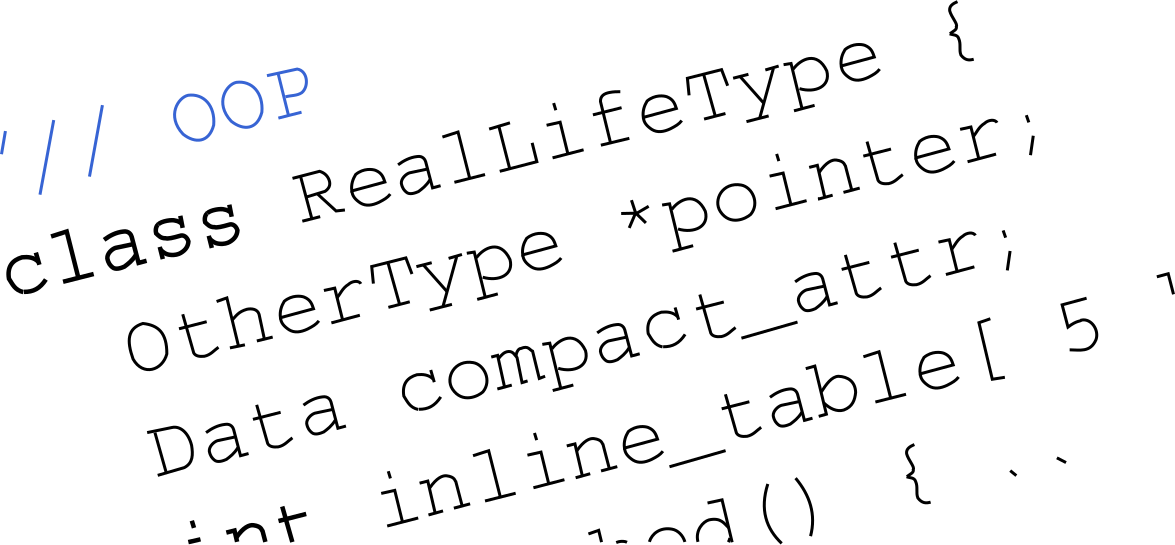
\includegraphics[width=0.3\textwidth]{img/class.pdf}
                \begin{center}
                \begin{scriptsize}
                    SocaDB gère en interne et de façon très efficace le typage et les indirections (pointeurs). Ceci permet d'accélérer considérablement le développement d'applications complexes, notamment celles faisant intervenir les \textit{motifs de conception} les plus courants.
                \end{scriptsize}
                \end{center}
            \end{wrapfigure}
        
            Sauf très rares exceptions, les applications modernes font toutes appel à des classes, pouvant utiliser des pointeurs, pouvant parfois se compacter de façon spectaculaire... mais peu de systèmes permettent de le prendre en compte de façon efficace.
            
            La tendance actuelle de se baser sur du JSON va précisément dans le sens inverse~: le JSON est intéressant pour le développement rapide d'applications simples, mais rend difficile et périlleux le développement d'applications plus complexes. Les bases de données type SQL sont un peu meilleures dans le sens où elles permettent une plus grande compacité au niveau du stockage, mais elles rendent par ailleurs très difficile et très inefficace le typage dynamique (par exemple pour la cohabitation d'objets de types différents).

            \medskip
            Un autre point important concerne l'évolutivité~: les applications évoluent, et logiquement, les formats de données aussi (par exemple le format des fichiers .doc est changé à chaque nouvelle version de Word). Pour une application de bureau, quand un nouveau format arrive, il suffit de fermer l'instance en cours pour charger la nouvelle version du programme. Pour les applications connectées et notamment pour les applications multi-composant (IoT, ...), l'histoire est tout autre. Il est hors de question de redémarrer tout le système (par exemple le système d'une ville entière) dès que le format d'une de ses applications a changé.
            
            Pour permettre aux applications de continuer à tourner même si le format des données produites a changé, \textbf{SocaDB propose de prendre en charge la conversion des nouveaux formats vers les anciens} et vice-versa, à travers des modules programmables par les développeurs. Cette fonctionnalité est fondamentale pour les \textbf{systèmes ouverts} et/ou au \textbf{fonctionnement ne pouvant tolérer d'interruption}.
        
        \subsection{Flexibilité}
        
            Comme expliqué dans les sections précédente, là où la quasi totalité de bases de données bloquent leurs choix pour cibler sur tel ou tel créneau, SocaDB permet pour chaque type de données de spécifier la façon de compresser, de transmettre, de modifier, de requêter...
            
            Dans un fonctionnement classique, les données temporelles devraient être stockées dans une base de données spécifiques (par exemple TempoDB), les données des utilisateurs dans un autre type de base de données (par exemple CouchBase), les don\-nées géographiques dans telle ou telle autre base de données... demandant à chaque fois du matériel et une gestion spécifique. SocaDB propose a contrario, une base générique de gestion du matériel, sur laquelle peuvent s'ajouter des greffons pour tel ou tel type de stockage, lié à tel ou tel type de requête, etc...
            
            Le niveau de flexibilité est donc considérablement plus important. \textbf{La cohabitation de différent choix peut fonctionner sans jamais nuire à la performance}.
        
        \subsection{Modèle de sécurité}
        
            Exception faite de Google Drive, de Firebase et de MeteorJS, les bases de données ne sont rarement voire jamais conçues pour gérer la sécurité des applications. Les bases de données comme MongoDB, Couchbase ou MySQL ne permettent pas en elle-même de dire si un \textit{document} (vs. une table) appartient à tel ou tel utilisateur, si ce document peut être lu ou modifié par un autre, etc.... Dans ce genre de cas, la logique de sécurité doit être programmée, ce qui en général est refait à chaque fois pour chaque nouvelle application, augmentant dans façon considérable le risque de failles, sans parler du temps perdu.
            
            \textbf{SocaDB gère la sécurité en interne}. Comme signalé dans les paragraphe précédents, il permet en outre de définir des règles de sécurité en fonction des types de données.
        
        \subsection{Traitements analytiques}
        
            Le premier endroit où les données du ``big data'' sont stockées, c'est dans les bases de donnée. L'interfaçage de bases de données avec les systèmes de calcul est donc d'importance considérable pour les acteur du domaine.
        
            %La thématique du ``big data'' ayant pris un importance considérable, sauf rares exceptions (Firebase par exemple) toutes les bases de données proposent des solutions pour les traitements analytiques.

            \medskip
            Sauf très rares exceptions (Firebase par exemple), toutes les bases de données proposent en fait des solutions pour les traitements analytiques...
            
            Mais quelques difficultés peuvent entacher cette promesse : la plupart des systèmes répartissent les données de façon aléatoire.
            
            SocaDB par contre cherche en permanence à positionner les données là où on en a le plus besoin (en vérifiant bien sûr qu'elles sont toujours bien copiées plusieurs fois). Cette fonctionnalité bénéficie en premier lieu à l'expérience utilisateur (comme le ferait un Content Delivery Network capable de gérer les écritures), mais aussi aux programmes de traitement automatiques qui de fait peuvent se retrouver plus près des données dont ils peuvent avoir besoin, minimisant les besoins en bande passante.
            
            %y compris dans le cas des bases de données les plus connues. Beaucoup centrent par exemple leurs traitements sur des modèles très spécialisés (par exemple, le modèle ``map-reduce'', très adapté pour la recherche, mais très contraignant pour d'autres cas). % SocaDB propose de signaler aux applications de calcul où sont situées les données, ces dernières pouvant prendre une décision en fonction des types d'algorithmes (alors que ``map-reduce'' a pour conséquence d'exécuter le même algorithme partout) et des mélanges de localisation de données (les traitements peuvent parfois se faire sur plusieurs ``tableaux'', dont les parties peuvent être à différents endroits).
        
            
            \medskip
            Un travail par ailleurs en cours pour simplifier le développement de requêtes complexes, en collaboration avec un laboratoire de recherche. Il s'agira en particulier de générer des graphes de taches, pour des requêtes exprimées de façon naturelles (avec les techniques de programmation usuelles). % Néanmoins, ce travail n'est pas terminé et il reste quelques défis à résoudre.
        
        \subsection{Interfaçages potentiels}
        
            Firebase, Google Drive ou MeteorJS sont chacun interfacés avec des librairies Javascript, Objective-C et Java pour la création d'interface utilisateurs simples pour le Web et les mobiles. Ces systèmes sont en effet conçus essentiellement dans ce but. Les liens vers l'internet de objets ou vers les applications de bureau ne semblent par contre pas à l'ordre du jour pour ce genre de bases de données (Google en particulier ne se positionne pas et ne se positionnera probablement jamais sur les applications de bureau).
            
            MongoDB, Couchbase ou MySQL de leurs côtés sont destinés à être utilisés via des middlewares, et l'absence de gestion de la synchronisation rend l'interfaçage direct avec ce genre de librairies sans intérêt.
        
            Les solutions comme RTI/DDS ou intersystems peuvent de leur côté prétendre fonctionner avec un nombre d'entités potentiellement beaucoup plus grand. Malheureusement, leur modèle de programmation, conçu pour le monde industriel, n'est pas vraiment adapté pour les autre cibles.
        
            \medskip
            L'efficacité des protocoles de SocaDB permet d'envisager \textbf{l'interfaçage avec une grande variété d'interfaces} (web, mobile, bureau, objets ou autre), une grande variété d'objets (capteurs, actionneurs physiques, ...) et de programmes de service. Ceci représente néanmoins un travail important, qui ne sera clairement pas réalisé de façon immédiate.
            
        \subsection{Gestion des ressources}

            \begin{wrapfigure}{r}{0.3\textwidth}
                \hfill
                \vspace{-0.9em}
                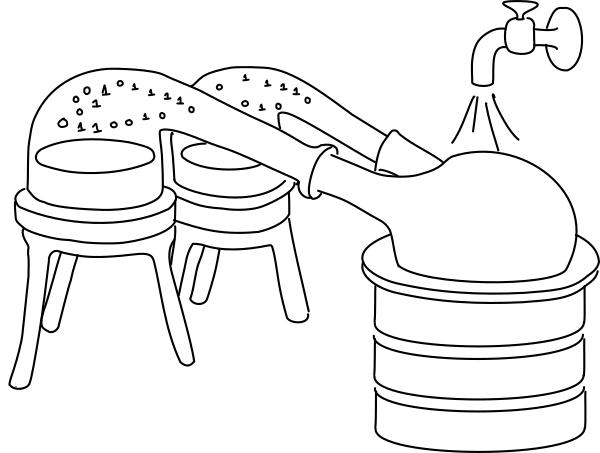
\includegraphics[width=0.3\textwidth]{img/distillation.pdf}
                \begin{center}
                \begin{scriptsize}
                    SocaDB est conçu du protocole à l'implémentation pour utiliser de façon optimale le stockage et la bande passante.
                \end{scriptsize}
                \end{center}
            \end{wrapfigure}

            Les implémentations de base de donnée ont toutes vocation à exploiter les ressources de façon optimale... mais en se basant sur des protocoles fixés, rarement voire jamais conçus pour aboutir à un tout optimisé. Les base de données basées sur du JSON ou équivalent ont les plus grandes difficultés à transmettre et stocker les données de façon efficace~: chaque donnée doit être associée à sa description, de sorte que les noms et les types (en général basiques et non extensible) se retrouvent copiés à côté de chaque donnée. Au sein de SocaDB, il existe une grande variété de types, et ceux-ci sont extensibles, de sorte qu'il est possible de parvenir à des stockages réellement compacts.
            
            
            Par ailleurs, le fait d'utiliser des middleware implique nécessairement des consommations supplémentaires.
            
            % Sur des exemples de données typées, nous avons pu constater des facteurs jusqu'à 40 concernant les besoins en terme de transmission et de stockage entre ce que permet SocaDB et les bases de données basées sur du JSON.
        
        \subsection{Confiance dans l'entreprise}
        
            Le modèle open-source de MongoDB ou SocaDB par exemple permet aux client de s'assurer que le code est de bonne qualité, et qu'il sera toujours disponible si l'entreprise change de politique commerciale. 
            
            D'un autre côté, des solutions comme RTI/DDS ne sont pas open-source mais sont utilisé par des clients très prestigieux, avec des cas d'utilisation assez spectaculaires. C'est clairement une autre façon de créer de la confiance, mais elle sera toujours limitée par le fait que les sources sont secrètes.
            
            Google (qui a racheté Firebase) de son côté ne donne pas les sources de ses programmes. L'entreprise est réputée pour la stabilité de ses produits, mais aussi pour utiliser de façon non documentée les informations sur ses clients. Les scandales successifs sur l'espionnage numérique ont sérieusement entamé la réputation du géant américain, éloignant un nombre significatif de client potentiels.
        
        \subsection{Simplicité du 1\up{er} tutoriel}
        
            La simplicité des premiers tutoriels est primordial pour l'adoption du plus grand nombre des développeurs. Malheureusement pour elles, les solutions industrielles, destinées avant tout à produire des codes efficaces et de qualité, demandent souvent la compréhension de concepts avancés avant de pouvoir démarrer quoi que ce soit. Sur ce niveau, SocaDB cherche a se situer près des concurrents tels que Firebase, mais la recherche d'efficacité concernant l'utilisation des ressources conduit à une exigeance sensiblement plus importante.
    
    % ----------------------------------------------------------------------------------------------------------------------------
    \section{Applications visées}

        La première cible de SocaDB est constituée par les développeurs d'applications ayant besoin d'un système de communication et de gestion de donnée... donc potentiellement tous les développeurs pour potentiellement tous les types d'application ne fonctionnant pas strictement en local.
        
        La cible est donc très large.
        
        %         Pour un résumé synthétique, la plupart des bases de données demandent aux développeurs un travail considérable de développement au sein de middlewares, ce qui expliquent le fait que peu d'applications de bureau sont aujourd'hui connectées de façon directe, et que le développement d'applications web et mobiles se retrouve souvent à être anormalement long. SocaDB propose de simplifier et d'accélérer significativement ces developpements.
        
        \medskip
        Nous proposons de segmenter la clientèle selon deux axes : domaine d'application et taille de l'entreprise cible.
            
        \subsection{Domaine d'application}

            Le domaine d'application va bien sûr influer sur les besoins et les priorités. Il est important aussi de noter que chaque domaine a ses usages, influencé quelques fois par des effets de mode.
            
            \subsubsection{Web}

                \begin{wrapfigure}{r}{0.3\textwidth}
                    \hfill
                    \vspace{-0.9em}
                    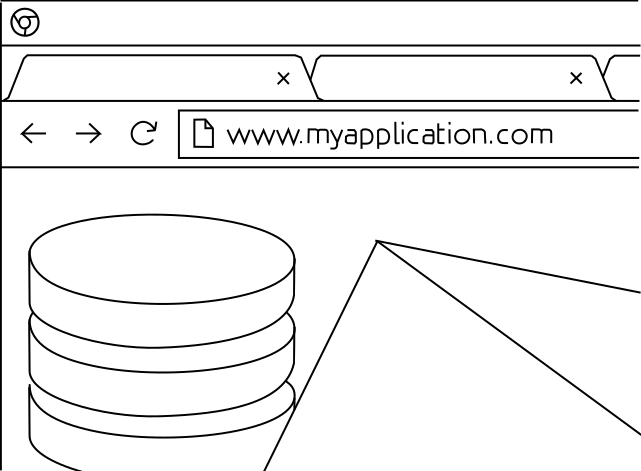
\includegraphics[width=0.3\textwidth]{img/webapp.pdf}
                    \begin{center}
                    \begin{scriptsize}
                        SocaDB permet de simplifier de façon considérable le développement d'applications Web interactives et collaboratives. Les applications javascript s'adressent directement et de façon sécurisée à la base de données.
                    \end{scriptsize}
                    \end{center}
                \end{wrapfigure}

                Les développeurs web forment la première cible, la plus évidente, et aussi la première qui permettra de générer du revenu. Le fonctionnement en ressources mutualisées oblige ces derniers à utiliser des bases de données pour gérer leurs informations. C'est un passage obligé. Les développeurs web auront un intérêt fort à utiliser SocaDB pour
                \begin{itemize}
                    \item la simplification extrême de leurs développements (qu'on peut rapprocher de ce que proposent MeteorJS ou Firebase). % -- nous avons du reste testé le codage d'applications web avec Ruby on Rails / MySQL versus SocaDB auprès de développeurs de profils différents, les version utilisant SocaDB ont demandé 5 à 6 fois moins de temps de développement.
                    \item l'ajout automatique du collaboratif temps-réel, qui correspond à un besoin fort, notamment dans le monde de l'entreprise où il arrive souvent que plusieurs personnes travaillent en même temps sur un même projet, le fonctionnement en séquentiel (les éditions de document se font chacun son tour) nuisant de façon considérable à la productivité.
                    \item l'exploitation optimale des ressources (bande passante, capacité de stockage, expérience client).
                \end{itemize}
                
                Les développeurs web sont particulièrement en demande de simplicité. Il faudra prendre garde à ce que cette dernière soit présente aussi bien pour les applications triviales (ce que font déjà très bien les middlewares et bases de données actuelles) que pour les applications riches, aux données et interfaces complexes.

                \medskip
                Par ailleurs pour être en mesure de générer rapidement du revenu, nous commencerons par exploiter nous même le système pour la création de sites et d'applications Web. Pour illustrer l'intérêt de SocaDB nous chercherons en priorité à répondre aux besoins en applications fortement interactives.
                
                Pour le démarrage, une des premières cibles sera donc les entreprises ayant besoin d'applications web.
                
            \subsubsection{Applications de bureau (pour Windows, Mac Os, Linux/KDE, ...)}
                
                Le fonctionnement en local, c'est à dire sans mutualisation des ressources, a jusqu'à présent suffit pour bon nombre d'applications de bureau. Néanmoins, le fonctionnement en multi-composants (comme décrit plus bas) et l'éducation du marché autour du collaboratif temps-réel va pousser les éditeurs de logiciels à connecter leurs applications de bureau. Ils auront besoin d'outils et il est clair que très peu sont disponibles pour ce marché (on pourra néanmoins citer Enginio Data Storage de Digia, associé à une communication assez limitée).

                % Les applications de bureau sont , tandis que l
                
                Le développement d'applications web en est encore au stade des balbutiements : très peu sont aussi puissantes, rapides, riches et conviviales que leur équivalent pour le bureau... mais la seule présence du collaboratif temps-réel à fait basculer des services entiers sur le web, renonçant au reste. SocaDB propose une solution pour gagner sur tous les tableaux.
                
                \begin{wrapfigure}{r}{0.3\textwidth}
                    \hfill
                    \vspace{-0.9em}
                    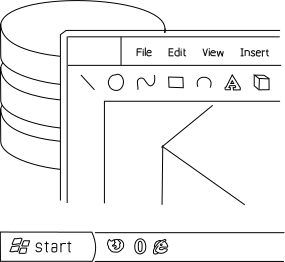
\includegraphics[width=0.3\textwidth]{img/windows.pdf}
                    \begin{center}
                    \begin{scriptsize}
                        SocaDB permet de connecter et de rendre collaboratives les applications de bureau. Une base de données ``locale'' permet d'atteindre de très grandes vitesses d'exécution, en plus de permettre le fonctionnement off-line.
                    \end{scriptsize}
                    \end{center}
                \end{wrapfigure}
                
                \medskip
                Les développeurs d'applications de bureaux auront donc intérêt à utiliser SocaDB pour
                    \begin{itemize}
                        \item la collaboration temps-réel, jusqu'à présent réservée à quelques applications web (et uniquement pour des données très simples comme du texte, ...);
                        \item les capacités de stockage et de résilience du cloud (tout en gardant la vitesse du local, SocaDB se basant sur le principe de serveurs locaux pour permettre le travail off-line et améliorer grandement l'expérience de l'utilisateur);
                        \item les capacités de calcul du cloud (en batch ou en temps-réel par exemple pour la visualisation et l'analyse de volumes conséquents de données).
                    \end{itemize}
                    
            \subsubsection{Applications multi-composant}
            
                \begin{wrapfigure}{r}{0.3\textwidth}
                    \hfill
                    %\vspace{-0.9em}
                    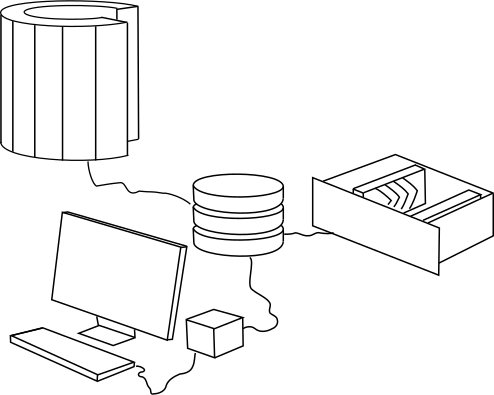
\includegraphics[width=0.3\textwidth]{img/distributed_computing.pdf}
                    \begin{center}
                    \begin{scriptsize}
                        SocaDB permet de développer de façon simple et sûre des applications multi-composants (des interfaces utilisateurs, des outils de calcul, des capteurs, des actionneurs physiques, etc...), potentiellement à grande échelle.
                    \end{scriptsize}
                    \end{center}
                \end{wrapfigure}
                
                SocaDB permet de gérer le \textbf{stockage et la communication ``réactive'' entre toutes sortes de composants} (interfaces utilisateurs, programmes de traitement automatique, objets connectés, ...).
            
                Si nous prenons l'exemple d'une \textbf{ville connectée}, on pourra commencer par remarquer que tout ce que propose une ville ne peut évidemment pas être géré par un seul et même ordinateur. SocaDB propose en pratique de gérer la communication entre toutes ces entités (avec possibilité de spécifier des contraintes sur la vitesse de transmission). Pour une autre exemple, cette fois-ci tiré de l'expérience actuelle de l'utilisation de SocaDB, on pourra citer la thématique de la \textbf{visualisation de volumes considérables de données}, etc...
            
        \subsection{Taille des entreprises}
        
            \subsubsection{Grosses entreprises}
            
                Les grosses entreprises utilisent en général des ressources internes aussi bien pour l'installation, le développement que pour la gestion du matériel. Les dévelop\-peurs et administrateurs y ont la responsabilité de pérenniser les données, en plus bien sûr de s'occuper de devoir optimiser l'utilisation des ressources tout en cherchant à améliorer l'expérience utilisateur. Ces derniers auront donc une forte propension à chercher des \textbf{formations}, et à \textbf{sécuriser} en sollicitant des \textbf{contrats de maintenance}.
                
                Dans le cas de très grosses entreprises, le rachat est par ailleurs est une possibilité souvent retenue pour être en mesure de maîtriser une technologie.
                    
            \subsubsection{Petites structures}
            
                Les petites structures seront plus à même de chercher des systèmes clé en main, en coût variable essentiellement. Pour ces dernières, il faudra donc proposer une offre flexible et facile d'accès, incluant potentiellement la \textit{location de matériel pré-installé} (comme le propose par exemple Firebase), et différentes catégories de formation.
    
    
    
% --------------------------------------------------------------------------------------------------------------------------------
% --------------------------------------------------------------------------------------------------------------------------------
% --------------------------------------------------------------------------------------------------------------------------------
\chapter{Moyens nécessaires à la maturation du projet}

    La figure ci-dessus décrit le déroulement des opérations sur les trois ans à venir :
    
    %    AXE TECHNO, ÉQUIPE, MARKETING

    \begin{center}
    \begin{ganttchart}[%
        time slot format=isodate-yearmonth,
        x unit=0.11mm,
        %         bar top shift=-0.1,
        group top shift=0.8,
        group height=0.05,
        bar height=0.55,
        %         milestone top shift=0.0,
        % %         milestone height=0.35,
        milestone left shift=-0.6cm,
        milestone right shift=0.6cm,
        % %         y unit title=.8cm,
        %         y unit chart=0.7cm,
        inline,
        milestone inline label node/.append style={right=1mm}
    ]{2015-02}{2018-12}
        \gantttitlecalendar{year} \\
        %         \ganttalignnewline
        %         \ganttmilestone{Première version publique}{2015-5} \\
        
        \ganttgroup{\color{MSBlue} Technologie }{2015-02}{2018-12} \\
        \ganttbar{Dev. lib. pour interfaces web}{2015-3}{2016-12} \\
        \ganttbar{Dev. outils big data et requêtes avancés}{2015-6}{2018-6} \\ % \ganttnewline[dotted, MSBlue]
        \ganttbar{Dev lib. pour Android/IOS/Qt}{2016-1}{2017-8} \\
        \ganttbar{Audit de sécurité}{2015-6}{2016-2} \\

        \ganttgroup{\color{MSBlue} Marché, propriété intellectuelle }{2015-02}{2018-12} \\
        \ganttbar{Brevets}{2015-02}{2016-1} \\
        \ganttbar{Offre développement sites web utilisant SocaDB}{2015-5}{2018-5} \\
        \ganttbar{Offres commerciales spécifiques pour SocaDB}{2016-6}{2018-12} \\ % \ganttnewline[dotted, MSBlue]
        \ganttbar{Business Angel(s)}{2016-1}{2017-1} \\ % \ganttnewline[dotted, MSBlue]
        \ganttbar{VC, 1\up{er} tour de table}{2017-1}{2018-1} \\ % \ganttnewline[dotted, MSBlue]
                
        
        % \ganttbar{Communication à grande échelle (blogs, salons, ...)}{2015-5}{2018-12} \\ % \ganttnewline[dotted, MSBlue]

        %         \ganttbar{}{2015-03}{2018-12} \\
        %         \ganttbar{}{2015-03}{2018-12} \\
        %         \ganttbar{}{2015-03}{2018-12} \\
        %         \ganttbar{}{2015-03}{2018-12}
    \end{ganttchart}        
    \end{center}

    
    

    % ----------------------------------------------------------------------------------------------------------------------------
    \section{Études à réaliser}
        % tecHnologique, d’organisation commerciale, financière, juridique
    
        Quelques premières recherches ont été effectuées autour des brevets existant ou à développer. Il sera néanmoins indispensable de passer par un cabinet spécialisé pour un travail plus en profondeur. Selon toute vraisemblance, le principe d'une base de donnée placée en position frontale pourrait être breveté. Le coût estimé pour cette première opération est de 5000\texteuro.
        
        \medskip
        Au niveau technologique, bien que tous les développements aient été réalisés de façon consciencieuse, il est possible que le produit présente encore des failles de sécurité, rédhibitoires pour la clientèle. Pour diminuer le risque, il conviendra donc de faire réaliser un audit de sécurité par une entreprise extérieure, et spécialisée. Un devis réalisé par la société nbs-system (cf. annexes) fait mention d'un montant de 14850\texteuro{} HT.
        
        \medskip
        Il faut bien sûr ajouter les études pour le dépôt de marque et le dépôt de status.
    
    % ----------------------------------------------------------------------------------------------------------------------------
    %     \section{Formation à apporter au candidat}
    %         Le candidat possède essentiellement les compétences techniques
    %     1000 lignes de code par jour -> 120 jours. audit durer 15 jours + prévoir 1.5 jours de rapport. 900€ jour homme.
    
    
    % ----------------------------------------------------------------------------------------------------------------------------
    \section{Partenariats existants ou à mettre en œuvre}
        % laboratoires publics, centres techniques, entreprises
        
        La vocation innovante de SocaDB conduit à aborder bon nombre de questions, dont certaines sont à la limite voire directement dans le domaine de la recherche. Par chance, certaines de ces questions sont abordées avec succès par la recherche française. Des collaborations sont donc en train de se mettre en place autour des thématiques suivante~: la compilation, l'ordonnancement et le calcul parallèle.
        
        Nous commençons en particulier par mettre en place un partenariat avec l'équipe MOAIS (\verb&http://moais.imag.fr&) dont Thierry Gautier, Chargé de Recherche à l'INRIA, est responsable. Les discussions pour définir un cadre de partenariat sont en cours (cf. mail en annexe).


    % ----------------------------------------------------------------------------------------------------------------------------
    \section{Planning des dépenses prévisionnelles}

        \subsection{Dépenses internes}

            Personnels permanent :
            \begin{center}
            \begin{tabular}{|m{0.75\textwidth}|R{0.15\textwidth}|}
                \hline
                Hugo Leclerc (porteur et architecte du projet). Feuilles de salaire à 0\texteuro{} pour cotisations retraite et sécurité sociale
                    & 500\texteuro/ mois ? \\
                \hline
                Associé technique  & ...\texteuro/mois \\
                \hline
                Associé commercial & ...\texteuro/mois \\
                \hline
            \end{tabular}
            \end{center}

            \medskip
            Personnels non permanent :
            \begin{center}
            \begin{tabular}{|m{0.75\textwidth}|R{0.15\textwidth}|}
                \hline
                Ingénieur développement javascript en CDD, pour les applications web et les prestations
                    & 5000\texteuro/mois \\
                \hline
                Ingénieur stagiaire javascript pour les interfaces développeurs et administration
                    & 436\texteuro/mois \\
                \hline
            \end{tabular}
            \end{center}
            
            \medskip
            Pour les dépenses internes, le cumul est de 71232\texteuro{} par an, dès la première année.
            
        \subsection{Dépenses externes}
        
            Matériel :
            \begin{center}
            \begin{tabular}{|m{0.75\textwidth}|R{0.15\textwidth}|}
                \hline
                Location de locaux adaptés (bureaux avec connection internet), éventuellement en pépinière si dossier non incubé
                    & 500\texteuro/mois \\
                \hline
                Location de serveurs en frais fixe pour documentation et démonstrateurs
                    & 215\texteuro/mois \\
                \hline
                Achat et installation du matériel informatique personnel
                    & 4500\texteuro \\
                \hline
                Location de serveurs en frais variables pour solutions de DBaaS (pas avant 2016, utilisation au plus près de besoins des clients)
                    & ...\texteuro \\
                \hline
            \end{tabular}
            \end{center}
            
            \medskip
            Prestations :
            \begin{center}
            \begin{tabular}{|m{0.75\textwidth}|R{0.15\textwidth}|}
                \hline
                Étude de propriété industrielle et dépôt des sources
                    & 4000\texteuro \\
                \hline
                Dépôt de brevet
                    & 5000\texteuro \\
                \hline
                Contrats avec graphistes pour le matériel de communication (site et démonstrateurs)
                    & 8000\texteuro \\
                \hline
                Encadrement administratif (comptabilité, droit)
                    & 200\texteuro/mois \\
                \hline
                Étude, rédaction et dépôt des statuts
                    & 3000\texteuro \\
                \hline
                Audit de sécurité
                    & 14850\texteuro \\
                \hline
            \end{tabular}
            \end{center}

            \medskip
            Pour la première année d'activité, le cumul est donc de 50330€ pour les dépenses externes.
        
            
% --------------------------------------------------------------------------------------------------------------------------------
% --------------------------------------------------------------------------------------------------------------------------------
% --------------------------------------------------------------------------------------------------------------------------------
\chapter{Caractéristiques de l’entreprise envisagée}
    % (à développer selon l'état d'avancement du projet)

    % ----------------------------------------------------------------------------------------------------------------------------
    %     \section{Besoins en locaux, en matériel...}
    
    % ----------------------------------------------------------------------------------------------------------------------------
    \section{Moyens financiers à mobiliser : besoins financiers et financements envisagés}
        % appOrt personnel, emprunts, fonds de capital d’amorçage, aides publiques, etc.
        
        50000\texteuro{} d'apports personnels.
        
        Aucune aide publique n'a été obtenue pour l'instant.

        Nous présenterons notre candidature à un prêt scientipôle-initiative pour constituer le fond de roulement.
        
        % Pas d'emprunts contracté pour l'instant, mais vu les calculs concernant la première année de fonctionnement, associé au peu de certitude concernant les prestations à réaliser, il semble pertinent de chercher vite à en négocier un. Nous projetons de nous porter assez vite candidats .
    
    % ----------------------------------------------------------------------------------------------------------------------------
    \section{Structure de l’entreprise envisagée}

        Pour mieux répondre aux besoins des investisseurs potentiels, il est envisagé de créer une structure de type SAS au capital initial de xxx \texteuro.



\end{document}          

 
